\documentclass[../../main.tex]{subfiles}
\begin{document}

{\bf [解答]}
対称性により，1回目に出た目を$1$として考える．
このとき，2回目から$n$回目までのサイコロの目の出方は$6^{n-1}$通りあり，いずれも同様に確からしい．
頂点$1$を含む直角三角形は，次の6個である．
\begin{align}
  (1,2,4)，\quad (1,2,5)，\quad (1,3,4)，\quad
  (1,4,5)，\quad (1,3,6)，\quad (1,4,6)．
\end{align}

\begin{figure}[htbp]
  \begin{center}
    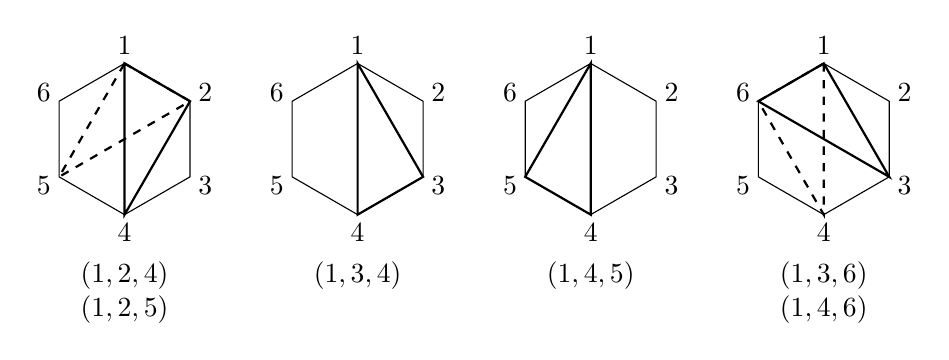
\begin{tikzpicture}[scale=0.8]
      \foreach \k in {0,1,2,3} {
        \begin{scope}[xshift=3.7*\k cm]
          \foreach \i in {1,...,6} {
            \coordinate (P\i) at ({90-60*(\i-1)}:1.2);
            \node at ({90-60*(\i-1)}:1.48) {$\i$};
          }
          \draw (P1) -- (P2) -- (P3) -- (P4) -- (P5) -- (P6) -- cycle;
          \ifnum\k=0
          \draw[thick] (P1) -- (P2) -- (P4) -- cycle;
          \draw[thick,dashed] (P1) -- (P2) -- (P5) -- cycle;
          \node[below,align=center] at (0,-1.8) {$(1,2,4)$\\$(1,2,5)$};
          \fi
          \ifnum\k=1
          \draw[thick] (P1) -- (P3) -- (P4) -- cycle;
          \node[below] at (0,-1.8) {$(1,3,4)$};
          \fi
          \ifnum\k=2
          \draw[thick] (P1) -- (P4) -- (P5) -- cycle;
          \node[below] at (0,-1.8) {$(1,4,5)$};
          \fi
          \ifnum\k=3
          \draw[thick] (P1) -- (P3) -- (P6) -- cycle;
          \draw[thick,dashed] (P1) -- (P4) -- (P6) -- cycle;
          \node[below,align=center] at (0,-1.8) {$(1,3,6)$\\$(1,4,6)$};
          \fi
        \end{scope}
      }
    \end{tikzpicture}
  \end{center}
  \caption{頂点$1$を含む直角三角形}
\end{figure}

\paragraph{(1)}

\subparagraph{$n=3$の時}

$n=3$のとき，三角形の残りの二つの頂点に対応する目をを一回ずつ出さなければならない．
三角形の数は$6$通り，どちらの目が先に出るかでそれぞれ$2$通りだから，合計の場合の数は
$6\cdot 2=12$通りである．よって求める確率は
\begin{align}
  p_3=\dfrac{12}{6^2}=\dfrac{1}{3}
\end{align}
である．

\subparagraph{$n=4$の時}

$n=4$のとき，直角三角形が存在しない目の出方は，\cref{eq:2}で示すように$84$通りであるから，
\begin{align}
  p_4=1-\dfrac{84}{6^3}=\dfrac{11}{18}
\end{align}
である．
\casesend

以上をまとめて
\begin{align}
  p_3 = \dfrac{1}{3}, \quad p_4 = \dfrac{11}{18}
\end{align}
である．

\paragraph{(2)}

余事象を考える．4個以上の異なる目が出れば，向かい合う頂点の対と，それ以外の頂点がしるしをもつため，必ず直角三角形が存在する．
したがって，直角三角形が存在しないのは，次のいずれかの場合である．

\begin{enumerate}
  \item 異なる目が2個以下しか出ない．
  \item 異なる目が3個出て，それらの頂点が直角三角形をつくらない．
\end{enumerate}

\subparagraph{異なる目が2個以下しか出ない時}

この場合は$1$以外の目を1個選び，残りの$n-1$回にその目が少なくとも1回出る場合と，すべて$1$が出る場合を合わせると，目の出方は
\begin{align}
  5(2^{n-1}-1)+1=5\cdot 2^{n-1}-4 \label{eq:1}
\end{align}
通りである．

\subparagraph{異なる目が3個出て，それらの頂点が直角三角形をつくらない時}

この場合，直角三角形にならない3個の目の組は
\begin{align}
  (1,2,3)，\quad (1,3,5)，\quad (1,5,6)，\quad (1,2,6)
\end{align}
の4組である．
例えば目の組が$(1,2,3)$となる場合の数を考える．
まずこの$3$つの目がでる場合の数は全体で$3^{n-1}$通りある．このうち$2$がでない場合と
$3$が出ない場合（いずれも$2^{n-1}$通り）を除き，両方とも出ない場合を戻して，
\begin{align}
  3^{n-1}-2\cdot 2^{n-1}+1
\end{align}
通りである．対称性から他の組み合わせも同じだけ場合の数があるから，合わせて
\begin{align}
  4(3^{n-1}-2^n+1) \label{eq:2}
\end{align}
通りある．
\casesend

以上\cref{eq:1,eq:2}より余事象が起こる確率$1-p_n$は
\begin{align}
  \begin{split}
    1-p_n
    &=\dfrac{5\cdot 2^{n-1}-4+4(3^{n-1}-2^n+1)}{6^{n-1}}\\
    &=\dfrac{-3\cdot 2^{n-1}+4\cdot 3^{n-1}}{6^{n-1}}\\
    &=4\Bigl(\dfrac{1}{2}\Bigr)^{n-1}
    -3\Bigl(\dfrac{1}{3}\Bigr)^{n-1}
  \end{split}
\end{align}
である．従って求める極限値は
\begin{align}
  \dfrac{1}{n}\log(1-p_n)
  &=\dfrac{1}{n}\log\Biggl\{
    4\Bigl(\dfrac{1}{2}\Bigr)^{n-1}
  \Bigl[1-\dfrac{3}{4}\Bigl(\dfrac{2}{3}\Bigr)^{n-1}\Bigr]\Biggr\}\\
  &=\dfrac{\log 4}{n}+\dfrac{n-1}{n}\log\dfrac{1}{2}
  +\dfrac{1}{n}\log\Bigl[1-\dfrac{3}{4}\Bigl(\dfrac{2}{3}\Bigr)^{n-1}\Bigr] \\
  &\xrightarrow{n\to\infty} -\log 2
\end{align}
となる．

\newpage

\end{document}
